\section{Implementing the \rt{} \pf{}}
\label{sec:particle-filter}


The next major step in this work was to implement the model in real-time using C++. Our implementation involves a single call from the R package \verb+transitr+ which commences an infinite loop within C++ which
\begin{enumerate}
\item fetches the lastest observations,
\item attaches them to an existing vehicle, or creates a new one,
\item updates or initialises vehicle states using the particle filter model described in \cref{sec:vehicle_model}, and
\item estimates average road speeds as vehicles traverse the network as described in \cref{sec:vehicle_speeds}.
\end{enumerate}
During the process of coding up our implementation (\cref{sec:pf_implementation}), we inevitably ran into issues, some of which are related to computational complexity, while others are due to imperfections with the data (see \cref{sec:pf_issues}). Once the implementation was complete, we needed to estimate the parameters (such as system noise and measurement error) for the model.


In order to assess the \rt{} performance of the model and our \pf{} implementation, we created a virtual \rt{} server which serves historical data. This means we can both process the data faster---we do not need to wait in \rt{} for new observations---and allows us to run the model with different settings and parameter values for comparison. We used (a subset of) data from Tuesday 8~October~2018 for the simulations used in \cref{sec:pf_issues,sec:pf_params}, which were carried out on a virtual machine with 8~Intel Xeon 3.00GHz CPU cores and 32~GB of memory, running Ubuntu 16.04 and R 3.4.1. The results themselves were processed locally using R 3.6.0. These results were published in \citet{Elliott_2020}.





\subsection{C++ particulars}
\label{sec:pf_implementation}

The general construction of the particle filter is straightforward and involves creating \class{Vehicle} and \class{Particle} objects (as well as the \gls{gtfs} objects described in \cref{sec:gtfs}). The \class{Vehicle} objects are stored within an \verb+std::unordered_map+ using their \gls{gtfs} \verb+vehicle_id+ as the key.

When a vehicle is first observed, a new \class{Vehicle} is created and inserted into the map. Then its state is initialised by creating a vector of $\Np$ \class{Particle} objects, each of which is assigned a speed between 0 and 30 m/s, and a distance based on the observation: for GPS observations, map matching is used to determine the approximate location, around which the particles are scattered. In situations where there are multiple candidate locations, particles are distributed uniformly between the minimum and maximum likely distances. For trip updates, the particles are placed at the appropriate stop. When new data for an existing vehicle is observed, the \class{Vehicle}'s relevant properties are updated (such as position and timestamp). Then each \class{Particle} is mutated using the transition function from \cref{sec:vehicle_model} and reweighted according to the likelihood function (\cref{sec:pf-likelihood}). If the effective sample size drops below the threshold $\Nthres=\frac{\Np}{4}$, the state is resampled with replacement and particle weights reset to $\frac{1}{\Np}$. See \cref{app:particle-resampling} for details on particle resampling.

Since the vehicles are modelled independently, and they only need to read from the \gls{gtfs} object (not modify it) the vehicle update step is easily parallelised to use $\tilde M$~cores using the \prog{OpenMP} library \citep{OMP}. This enables up to an $\tilde M$-fold increase in the speed of this step.

Once the update is complete, the segment index of all particles is obtained, and the \emph{minimum} is used as the vehicle's \emph{current segment}. If this is greater than it was at the end of the previous iteration, the average speed along all intermediate segments is computed by using \verb+std::accumulate+,
\begin{lstlisting}
double avg_speed = std::accumulate(state.begin (), state.end (), 0.0,
  [](double x, Particle& p) {
    return x + p.weight () * p.segment_speed.at (seg_index);
  });
\end{lstlisting}\pagebreak
along with the variance,
\begin{lstlisting}
double var_speed = std::accumulate(state.begin (), state.end (), 0.0,
  [&avg_speed](double x, Particle& p) {
    return x + p.weight () *
      pow (p.segment_speed.at (seg_index) - avg_speed, 2.0);
  });
\end{lstlisting}
These observations are then passed to the relevant \class{Segment} object which contains a vector of new data (used in chapter 4). The \class{Vehicle} object contains a pointer to its \class{Trip}, which has a list of \class{Segment} objects:\footnote{Note that we must still ensure each pointer exists before proceeding, as mentioned in \cref{sec:rt-implementation}.}
\begin{lstlisting}
trip ()->segments ().at (seg_index)->push_data (avg_speed, var_speed);
\end{lstlisting}

At this point, we have completed the modelling of the vehicle's state and obtained estimates of any available road speed information.

\subsection{Real-time performance of the \pf{}}
\label{sec:pf_issues}



The two components of the model to assess are the iteration timings and the performance of the particle filter itself. That is, does the program run fast enough to be feasible in real-time, and is the model (and its \pf{} implementation) capable of modelling transit vehicles in real-time?


\paragraph{Is the particle filter fast enough?}
At peak hour on a typical weekday morning, there can be in excess of 1000~buses operating in Auckland. This leads to having more than $1000\Np$~particles in memory, each being mutated and reweighted approximately once every 30~seconds or so. By varying $N$, we can control how quickly each set of observations is processed. \Cref{fig:pf_timings} shows the average timings of the vehicle model component of our application, as well as the average time per particle for varying $N$. More particles require more processing power, though there is additional overhead during the \emph{resampling} phase. Limiting the frequency of resampling is therefore necessary to make the program run faster, which is why we use the effective sample size, $\Neff$, described in \cref{sec:pf} on \cpageref{eq:Neff}.


\begin{knitrout}\small
\definecolor{shadecolor}{rgb}{0.969, 0.969, 0.969}\color{fgcolor}\begin{figure}

{\centering 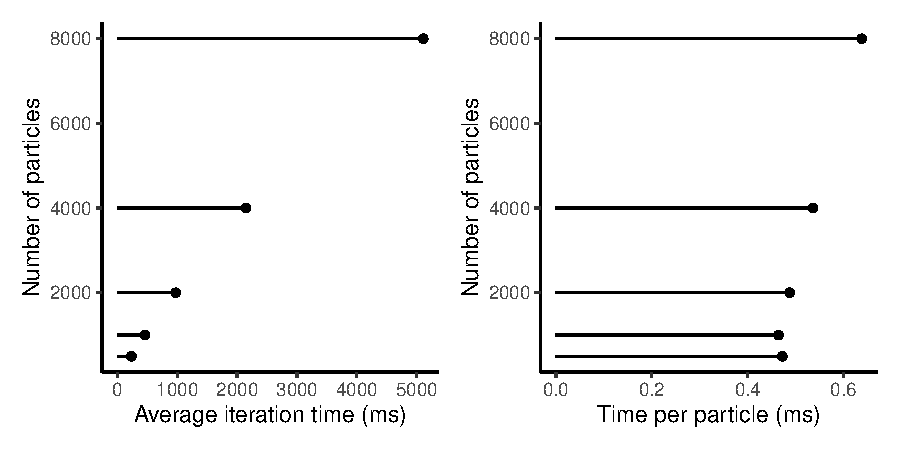
\includegraphics[width=.8\textwidth]{figure/pf_timings-1} 

}

\caption[Timings of the particle filter implemention for varying number of particles]{Timings of the particle filter implemention for varying number of particles. Left: the average iteration time (wall clock). Right: the average time per particle.}\label{fig:pf_timings}
\end{figure}


\end{knitrout}


\paragraph{How does the model perform?}





To assess how well our model performs in real-time, we repeated the simulation with a range of values of system noise $\Vnoise$, \gls{gps} error $\GPSerr$, and the number of particles $\Np$. For each simulation, we computed \emph{proportional effective sample size}, \emph{degeneration rate}, and \emph{relative variance}.

The \emph{proportional effective sample size} is the effective sample size relative to $N$, $\tilde N_\text{eff} = \frac{\Neff}{\Np}$. The higher this value, the less often the vehicle's state needs resampling, decreasing the average iteration time. \Cref{fig:model_performance_neff} shows the effect of $\Np$, system noise, and \gls{gps} error on $\tilde N_\text{eff}$. The most striking relationship is between $\tilde N_\text{eff}$ and \gls{gps} error: for larger error, more particles retain a high likelihood, and so the total weight is more evenly distributed. Conversely, larger values of system noise result in more variation between particles, leading to fewer particles ending near the observation position and decreasing $\tilde N_\text{eff}$.

\begin{knitrout}\small
\definecolor{shadecolor}{rgb}{0.969, 0.969, 0.969}\color{fgcolor}\begin{figure}

{\centering 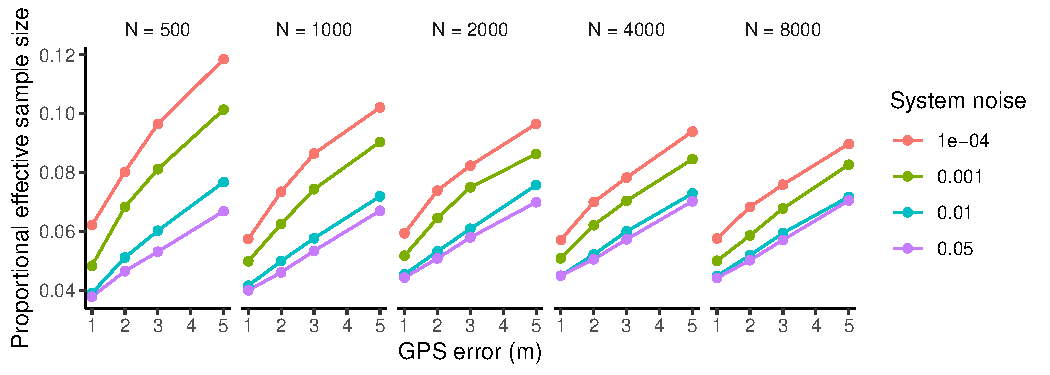
\includegraphics[width=\textwidth]{figure/model_performance_neff-1} 

}

\caption[Proportional effective sample size for varying values of GPS error, system noise, and number of particles]{Proportional effective sample size for varying values of GPS error, system noise, and number of particles.}\label{fig:model_performance_neff}
\end{figure}


\end{knitrout}


The \emph{degeneration rate} is the proportion of samples in which no particles end near the vehicle's reported position. In this case, all the particle likelihoods tend to zero, so the weights become undefined, resulting in the need to reinitialise the vehicle's state which results in the loss of any vehicle speed information along the most recently travelled road segment(s). We see from \cref{fig:model_performance_degen} that increasing \gls{gps} error or the number of particles reduces degeneration rate while increasing system noise shows a negligible reduction in degeneration rate. Larger \gls{gps} error means that particles do not need to end as close to the observed location to have a positive likelihood while increasing $\Np$ means more chance for a particle to end near the true bus.

\begin{knitrout}\small
\definecolor{shadecolor}{rgb}{0.969, 0.969, 0.969}\color{fgcolor}\begin{figure}

{\centering 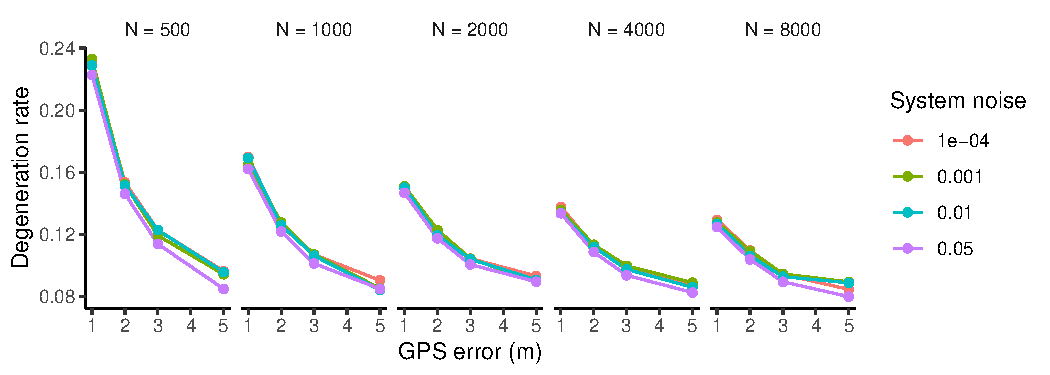
\includegraphics[width=\textwidth]{figure/model_performance_degen-1} 

}

\caption[Degeneration rate for varying values of GPS error, system noise, and number of particles]{Degeneration rate for varying values of GPS error, system noise, and number of particles.}\label{fig:model_performance_degen}
\end{figure}


\end{knitrout}

Finally, we have \emph{relative speed variance} along roads, which we use to compare the precision of the various models. It is the ratio of variance for a single simulation compared to the overall variance for all simulations. Let $\vec z_\ell^{e,s}$ be a vector of all vehicle speeds along road segment $\ell$ during the simulation with \gls{gps} error and system noise equal to $e$ and $s$, respectively. The ratio of the variance of speed for the single simulation compared to all simulations along one single road segment is given by
\begin{equation}
\label{eq:rel_speed_var_ratio}
v_\ell^{e,s} =
\frac{
    \mathrm{Var}(\vec z_\ell^{e,s})
}{
    \mathrm{Var}(\cup_e\cup_s \vec z_\ell^{e,s})
}.
\end{equation}
That is, for each segment in each simulation, we have a value representing whether this simulation estimates speed more or less accurately. We then compute the average ratio for all $L$ road segments,
\begin{equation}
\label{eq:rel_speed_var}
\bar v^{e,s} = \frac{1}{L} \sum_{\ell=1}^L v_\ell^{e,s}.
\end{equation}
A small value of $\bar v^{e,s}$ tells us that, on average, the simulation with \gls{gps} error $e$ and system noise $s$ estimates road speed \emph{with greater precision} than the other simulations. \Cref{fig:model_performance_var} presents these results, where we see the greatest effect on relative variance caused by increasing \gls{gps} error. Increasing $\Np$ produces a small decrease, and changes to system noise show no discernible effect.


\begin{knitrout}\small
\definecolor{shadecolor}{rgb}{0.969, 0.969, 0.969}\color{fgcolor}\begin{figure}

{\centering 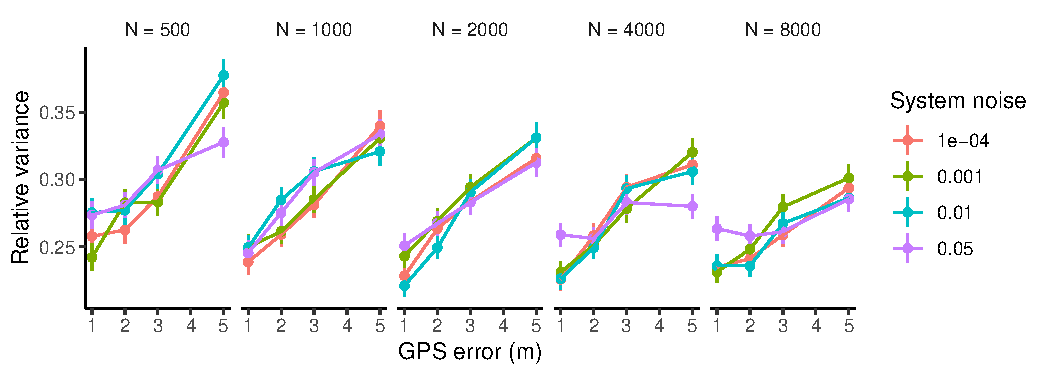
\includegraphics[width=\textwidth]{figure/model_performance_var-1} 

}

\caption[Relative speed variance for varying values of GPS error, system noise, and number of particles]{Relative speed variance for varying values of GPS error, system noise, and number of particles.}\label{fig:model_performance_var}
\end{figure}


\end{knitrout}


The results displayed in \cref{fig:model_performance_neff,fig:model_performance_degen,fig:model_performance_var} present a \emph{trade-off} between performance and estimation. Increasing \gls{gps} error increases the effective sample size, which reduces the frequency of resampling and speeds up each iteration. We also see a reduction in the rate of degeneration, which implies the particle filter is less likely to lose the vehicle and provide the desired speed estimates. However, increasing \gls{gps} error also increases the relative uncertainty of speed estimates. Increasing the number of particles generally results in a reduction in both degeneration rate and relative uncertainty, but, from \cref{fig:pf_timings}, this comes at the cost of increased computational demand.

\subsection{Handling invalid data in real-time}
\label{sec:data_issues}

Much of the degeneration or \emph{vehicle loss} can be attributed to irregularities with the incoming real-time data. There are two leading causes of this, described below, which can be detected and potentially avoided with a similar solution.


\paragraph{Buses that appear to go backwards}

One of the prominent assumptions of our model is that the bus cannot go backwards along the route, which is implemented by only allowing for non-negative values of speed. However, a couple of scenarios can lead to the \emph{appearance} of a reversing bus, both of which are related to \emph{\gls{gps} waypoints}; that is, the \gls{avl} systems in Auckland Transport's buses are programmed to not only report their position periodically but also to report their arrival at certain waypoints. These can include bus stops (which result in an arrival or departure time update) as well as some major intersections. The issue is that, rather than reporting the bus's \gls{gps} position, they report the \gls{gps} coordinates of the waypoint itself. This is often acceptable since the bus continues straight past the intersection or bus stop before reporting another position. However, if there is congestion leading into the waypoint, the bus may:
\begin{enumerate}[i.]
\item approach the waypoint, decide it has arrived, and report its position \emph{at the waypoint},
\item get stopped in a queue for some time,
\item decide it is time for another position update, based on its GPS position.
\end{enumerate}
\Cref{fig:bus_going_backwards} presents an example of this.

\begin{knitrout}\small
\definecolor{shadecolor}{rgb}{0.969, 0.969, 0.969}\color{fgcolor}\begin{figure}

{\centering 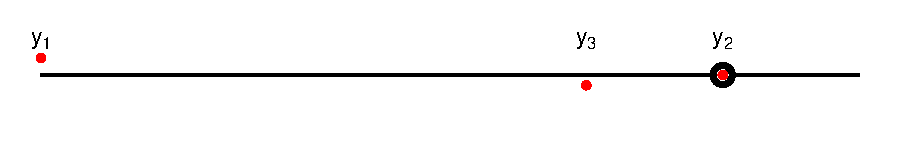
\includegraphics[width=.8\textwidth]{figure/bus_going_backwards-1} 

}

\caption[Visual demonstration of the ``reversing bus'' phenomenon]{Three sequential observations of a vehicle approaching an intersection (hollow circle). When the bus nears the intersection, it reports its position exactly at the intersection ($\Vobs_2$); however, there is a queue at this intersection, so the next observation ($\Vobs_3$) is behind the previous one, demonstrating the ``reversing bus'' phenomenon.}\label{fig:bus_going_backwards}
\end{figure}


\end{knitrout}


The effect this has on the \pf{} is that, after observing $\Vobs_2$, the vehicle's state (represented by a sample of particles) will all be around the intersection. On receiving the next observation $\Vobs_3$, the particles are transitioned \emph{forward} by $(\Vtime_3 - \Vtime_2)$~seconds, which places them at or beyond the intersection; none of the particles will be near observation $\Vobs_3$ and will likely all have a likelihood of zero. In this case, the particle filter has degenerated and needs reinitialising.


A similar situation occurs when approaching a bus stop that has an intersection just before it. Here, the bus gets stopped at the intersection, but not before reporting its position at the stop since it was almost there. A subsequent observation then shows the bus at the intersection, which again appears to involve a reversing bus. The main issue we face is that \emph{we do not know the location of intersections} since there is no easily accessible data for this.\footnote{We presented an intersection model, but this was more of a demonstration of flexibility, not of functionality.}


Checking for the bus-reversing scenario in real-time requires mapping of observations onto the route shape; that is, the \emph{inverse measurement function}, allowing us to detect if the bus has gone backwards:
\begin{equation}
\label{eq:vehicle_rev_check}
\Vmeas^{-1}(\Vobs_k) < \Vmeas^{-1}(\Vobs_{k-1}).
\end{equation}
Of course, the inverse function is not exact, since the true location is unlikely to be positioned exactly on the line (roads have width, and \gls{gps} devices have error). To compute $\Vmeas^{-1}$, we find the shortest distance along the route's shape that is closer than a threshold of $3\GPSerr$, which allows for situations where the route passes the observed location point more than once (such as in loops).

If the observation is determined to be going backwards, we have to decide between
\begin{enumerate}[i.]
\item ignoring the current observation, or
\item ignoring the previous observation and restoring the vehicle's previous state.
\end{enumerate}
If we can determine that the first observation is a pre-emptive observation (that is, at a waypoint), then option (ii) is the logical choice, although this requires storing each vehicle's state \emph{twice}. Otherwise, it is easier to ignore the current observation completely and use option (i). Note that, were intersection locations knowable, we could include this behaviour in the model; as it stands, however, this workaround is required to avoid unnecessary degeneration.


\paragraph{Buses that remain stationary}

Another situation (which can also occur around unknown intersections) is when the bus does not move between successive observations (or it moves very slowly). For example, the bus may need to turn onto a major road, for which there is a queue of traffic. The bus will report its position when it arrives, and may again report its position after moving a few meters. If our model does not allow for the bus to suddenly slow down in these situations, the particles will all be far ahead of the bus and degeneration will occur.


We can determine if the bus has remained more-or-less stationary by computing the distance between successive observations and comparing to a threshold:
\begin{equation}
\label{eq:vehicle_dist_check}
\dist{\Vobs_{k-1}, \Vobs_k} < \distThreshold =
\Vtdiff_k \min_i\left(\Vspeed_k\vi\right).
\end{equation}
The threshold here is the expected distance travelled in $\Vtdiff_k$~seconds by the slowest particle. Rather than slowing the particles (which could run into the opposite problem once the vehicle passes through the intersection), we sample a temporary speed,
\begin{equation}
\label{eq:vehicle_temp_speed}
\Vspeed_k\vi \sim
\Uniform{0}{\frac{\dist{\Vobs_{k-1}, \Vobs_k}}{\Vtdiff_k}},
\end{equation}
which is used for one single iteration.

Again, if we knew the locations of intersections, we could integrate this behaviour into the model. Particles could partake in ``creeping'' up to the intersection, before quickly accelerating back up to speed on the next road segment. Even then, however, the above behaviour would still need to be included to handle non-intersection related slowing down, for example, when reaching a congested section of a road.

\subsection{Parameter selection}
\label{sec:pf_params}

Once the inherent data issues have been dealt with,
we can begin determining the values of the model parameters.
Some of these are fixed and constant across all vehicles, routes, and stops,
for example,
GPS error, $\GPSerr$,
system noise, $\Vnoise$,
and minimum dwell time, $\mindwell$.
Others will inevitably vary between routes, stops, and time of day,
such as stopping probability, $\Prstop$,
and dwell time, $\dwell$.


% We explore these by modelling a subset of routes throughout Auckland over several days,
% using historical data to allow us to vary parameters and compare their effects.
% Some parameters, notably $\GPSerr$ and $\dwell$
% can be determined from the data:
% the value $\GPSerr$ can be approximated by looking at the variability
% of points around the route,
% since we assume there is no directional bias,
% so the distance from an observation to the route is an approximate estimate
% of measurement error.


\subsubsection{GPS error}
\label{sec:pf_params_gps}

The GPS or \emph{measurement} error used in the model has a strong effect on performance, as we saw in \cref{sec:pf_issues}. We can get a simple estimate of GPS error by examining the distribution of observations around the route; that is, we computed the shortest distance between the route and each observation, and graphed the results in \cref{fig:pf_param_gps}. We see two modes at about 0.5 and 2.5~meters, which could be due to a multitude of reasons. One likely one, however, is \emph{road width}, since the route shapes typically run in the middle of the road and the buses drive either side of the center line. Single-lane roads will have a smaller average distance between the bus and the center line, while for roads with two or more lanes, this will be larger. Additionally, some roads have a median (either painted or raised) which further increases the distance between the bus and the ``center line''. It is possible that some combination of this could result in the distribution shown in \cref{fig:pf_param_gps}.



\begin{knitrout}\small
\definecolor{shadecolor}{rgb}{0.969, 0.969, 0.969}\color{fgcolor}\begin{figure}
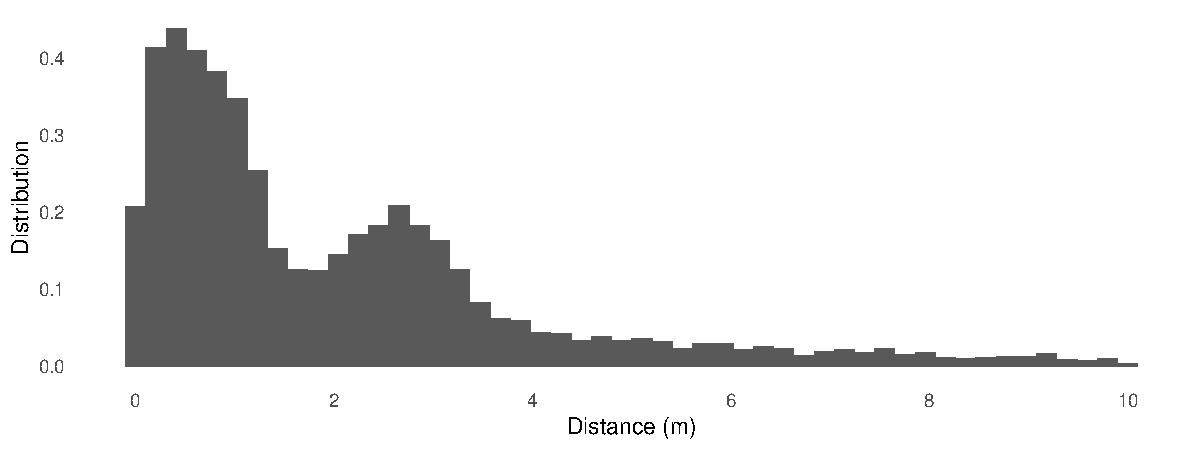
\includegraphics[width=\maxwidth]{figure/pf_param_gps-1} \caption[Distribution of distance from observation to nearest point on the route, truncated to 10~m]{Distribution of distance from observation to nearest point on the route, truncated to 10~m.}\label{fig:pf_param_gps}
\end{figure}


\end{knitrout}

The other issue is the heavy tail in the distribution of distance to path, which we trunctated to 10~meters to more easily see the modes. GPS devices usually have good accuracy, but occasionally they may be quite far off of the true location, possibly due to physical interference. 6\% of bus observations were more than 10~meters from the shape, excluding any observations greater than 50~meters since these were most likely attributed to the wrong trip (and therefore not anywhere near the route path). This would explain a large proportion of the degeneration rate (\cref{fig:model_performance_degen}), which we saw previously decreases significantly with increased GPS error.





\subsubsection{System noise}
\label{sec:pf_params_noise}

The definition of system noise is model-dependent; for transition models $f_{A1}$ and $f_{A2}$ it is \emph{the average change in speed per second}, while for model $f_{A3}$ it is \emph{the average change in acceleration per second}. From the simulations in \cref{sec:pf_issues}, we demonstrated that system noise affected the performance of the particle filter (how often resampling is required) but neither the degeneration rate nor parameter estimation.

Unlike GPS error, it is not possible to estimate system noise directly from the data. Indeed, most of the time a vehicle's speed is constant, but may change suddenly at certain locations (which are unknown), so the system noise must allow for this. We found that a smaller value of system noise under the second transition model $f_{A2}$ gave the best results in terms of sampling possible trajectories, and as such this was the model used during the simulation.



\subsubsection{Dwell times}
\label{sec:pf_params_dwell}

We are able to observe a large proportion of dwell times at stops, by compiling all those for which we have observed both arrival times $\Varr_{srm}$ and departure times $\Vdep_{srm}$ at stop $m$ of trip $r$ on day $s$ giving us a set of dwell times
\begin{equation}
\label{eq:dwell_time_obs}
\Vdwell_{srm} = \Vdep_{srm} - \Varr_{srm}
\end{equation}

\begin{knitrout}\small
\definecolor{shadecolor}{rgb}{0.969, 0.969, 0.969}\color{fgcolor}\begin{figure}
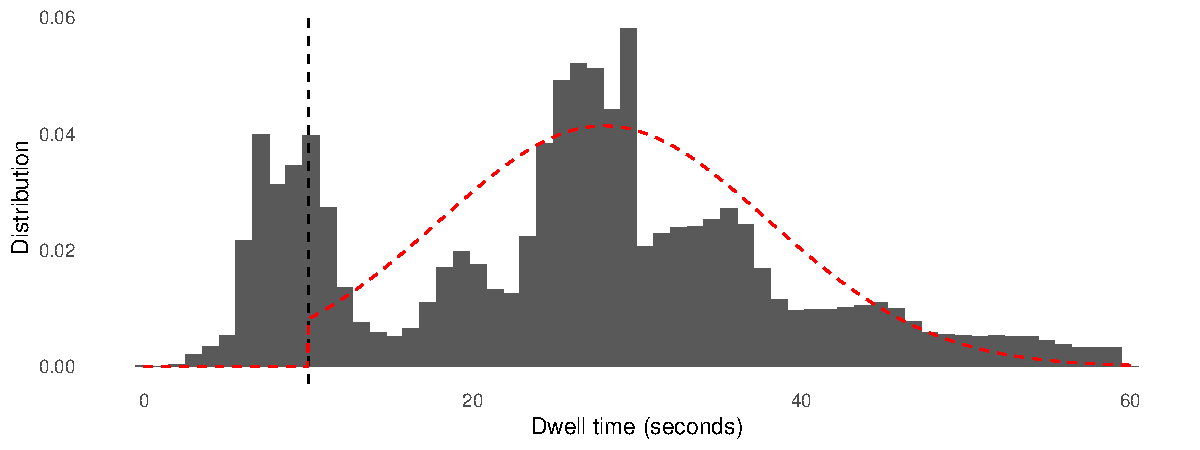
\includegraphics[width=\maxwidth]{figure/observed_dwell-1} \caption[Distribution of dwell times observed over the course of five days, truncated at one minute]{Distribution of dwell times observed over the course of five days, truncated at one minute.}\label{fig:observed_dwell}
\end{figure}


\end{knitrout}

There is no precise way to measure the minimum dwell time parameter $mindwell$. \cite{Hans_2015} used $\mindwell = 6$~seconds, which is marked by a dashed vertical line in \cref{fig:observed_dwell}. There are a few dwell times less than this, but given the spike at 6~seconds, it seems reasonable to continue with this value.

The raw data from five~days' observations are shown in \cref{fig:observed_dwell}. Here, we see an interesting pattern with apparent peaks every nine~seconds. While we could not determine the precise cause, we assume it to be due to a systematic problem in the arrival time recording system used to collect the data. From the historical dwell time data, we were able to estimate the mean and variance of dwell time for each stop $j$, $\bar\dwell_j$ and $\dwellvar_j$, respectively, which could then be used in the dwell time model.


The dwell times for each stop calcualted above \emph{include} the minimum dwell time phase. To avoid having to recompute each stop's dwell time parameter whenever $\mindwell$ is changed, we adjusted the mean of each stop's dwell time at run time to account for the minimum dwell time. That is, we use $\dwell_j = \bar\dwell_j - \mindwell$ in \cref{eq:stop_dwell_time}.

